% label C_\pm on fig 2
% unify 3 & 4, choose consistent q/cos q
    \documentclass[
        fleqn,
        usenatbib,
        referee,
    ]{mnras}
    \usepackage{
        amsmath,
        amssymb,
        newtxtext,
        newtxmath,
        graphicx,
        ae, aecompl,
        booktabs,
        caption,
        subcaption,
    }
    \usepackage[T1]{fontenc}
    \captionsetup{compatibility=false}

    \newcommand*{\rd}[2]{\frac{\mathrm{d}#1}{\mathrm{d}#2}}
    \newcommand*{\rtd}[2]{\frac{\mathrm{d}^2#1}{\mathrm{d}#2^2}}
    \newcommand*{\pd}[2]{\frac{\partial#1}{\partial#2}}
    \newcommand*{\md}[2]{\frac{\mathrm{D}#1}{\mathrm{D}#2}}
    \newcommand*{\at}[1]{\left.#1\right|}
    \newcommand*{\abs}[1]{\left|#1\right|}
    \newcommand*{\ev}[1]{\langle#1\rangle}
    \newcommand*{\bm}[1]{\boldsymbol{\mathbf{#1}}}
    \newcommand*{\p}[1]{\left(#1\right)}
    \newcommand*{\s}[1]{\left[#1\right]}
    \newcommand*{\z}[1]{\left\{#1\right\}}
    \DeclareMathOperator*{\argmin}{argmin}
    \DeclareMathOperator*{\argmax}{argmax}
    \DeclareMathOperator*{\med}{med}

\title[Analytical Exoplanet Obliquities]{Analytical Predictions of Explanet
Obliquities Generated by Planet-Disk Interactions}
\author[Y. Su and D. Lai]{
Yubo Su$^1$,
Dong Lai$^{1,2}$
\\
$^1$ Cornell Center for Astrophysics and Planetary Science, Department of
Astronomy, Cornell University, Ithaca, NY 14853, USA
\\
$^2$ Tsung-Dao Lee Institute, 800 Dongchuan Road, Shanghai, 200240, China
}

\date{Accepted XXX\@. Received YYY\@; in original form ZZZ}

\pubyear{2020}

\begin{document}\label{firstpage}
\pagerange{\pageref{firstpage}--\pageref{lastpage}}
\maketitle

\begin{abstract}
    Abstract here
\end{abstract}

\begin{keywords}
planet--star interactions % chktex 8
\end{keywords}

\section{Introduction}

Separatrix crossing was studied by \citep{henrard1982}.

\section{Theory and Equations}\label{s:theory}

We study an oblate planet orbiting around a star hosting a further out planet.
The equations of motion in the absence of dissipation are:
\begin{align}
    \rd{\hat{s}}{t}
        &= \omega_{s1}\p{\hat{s} \cdot \hat{l}_1}\p{\hat{s} \times \hat{l}_1}
            - \omega_{1p}\cos I\p{\hat{s} \times \hat{l}_p},\\
    \omega_{s1} &= \frac{3k_q}{2k}\frac{M_*}{m_1}\p{\frac{R_1}{a_1}}^3 s,\\
    \omega_{1p} &= \frac{3m_p}{4m_*}\p{\frac{a_1}{a_p\sqrt{1 - e_p^2}}}^3 \Omega_1.
\end{align}

We define $s_c$ to be the critical spin where the precession frequencies
$\omega_{s1}$ and $\omega_{1p}$ are equal, or
\begin{equation}
    \at{\omega_{s1}}_{s = s_c} = \omega_{1p}\cos I.
\end{equation}
rhroughout this paper, we often set the orbital frequency of the inner planet
$\Omega_1 = 1$.

\subsection{Cassini States}\label{ss:cs_theory}

Equilibria of spin dynamics are \emph{Cassini States} (CSs). Refer to Su \& Lai
2020 for more detailed discussion. In the notation of the previous paper,
\begin{equation}
    \eta \equiv -\frac{g}{\alpha} = s_c / s.
\end{equation}

Plots of CS locations as always in \autoref{fig:cs_locs}.
\begin{figure}
    \centering
    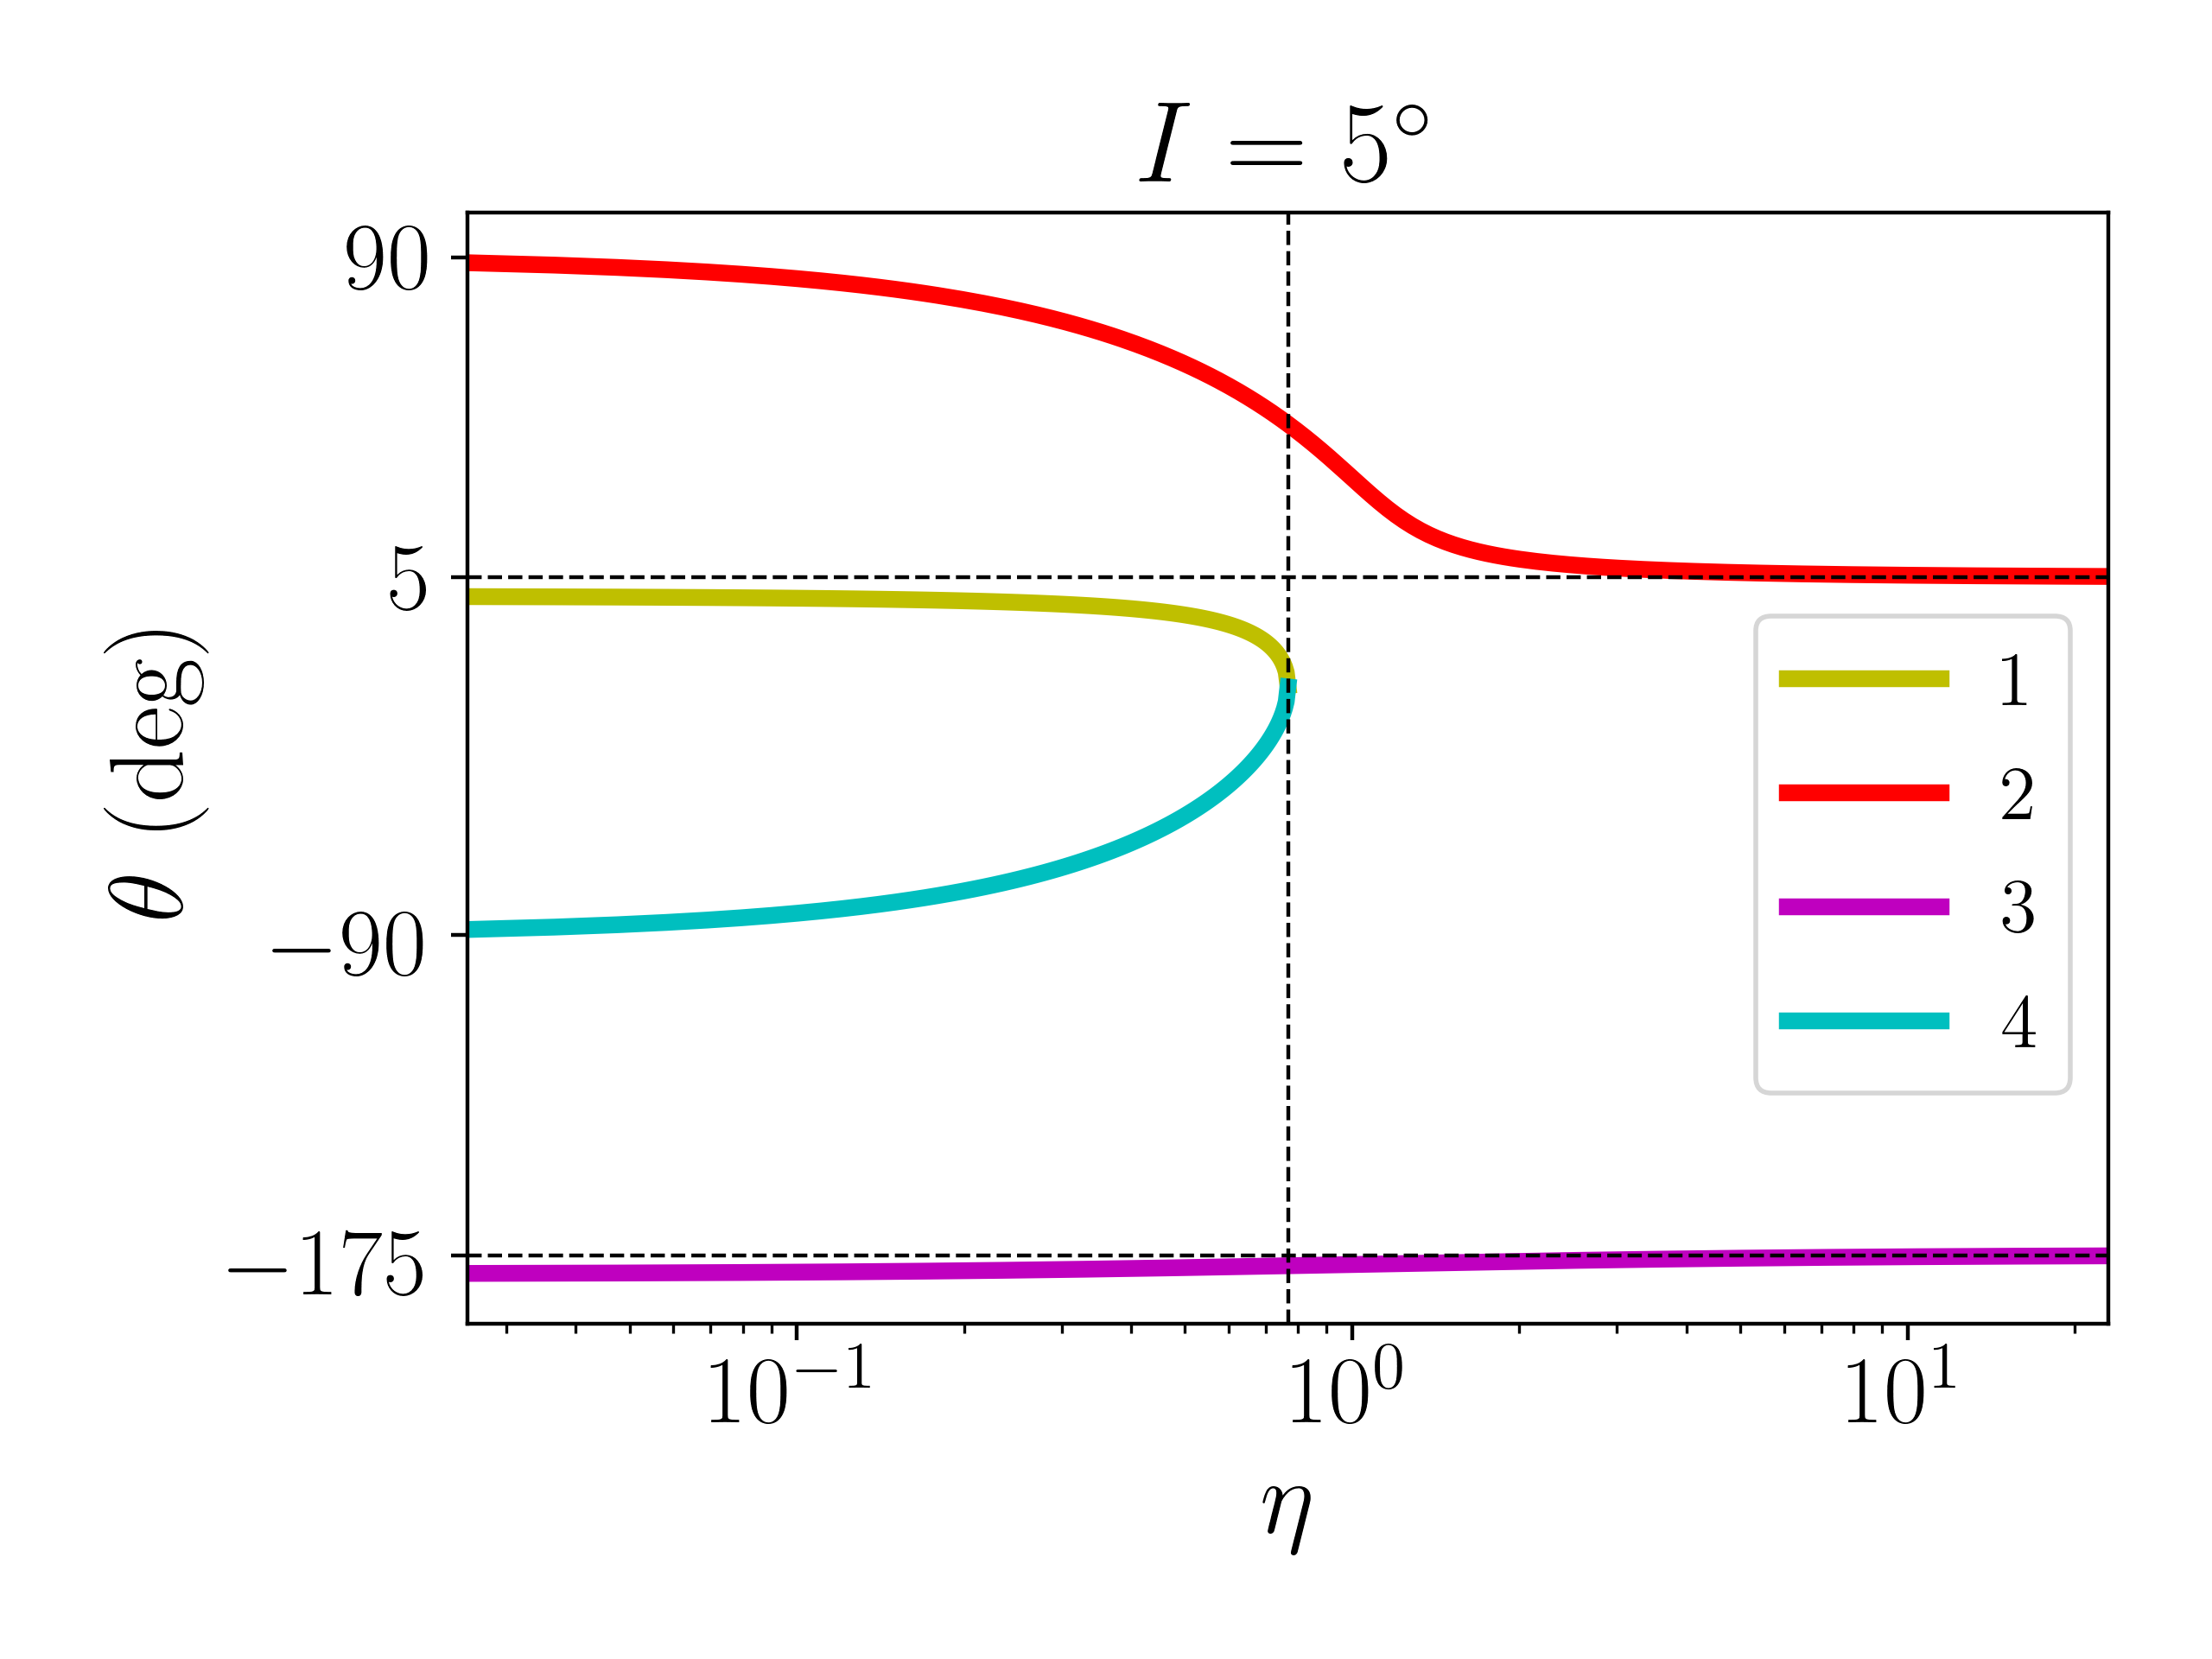
\includegraphics[width=0.6\textwidth]{../initial/99_misc/2_cs_locs.png}
    \caption{CS locations, TODO change axis labels etc.}\label{fig:cs_locs}
\end{figure}

Note that $\phi$ is conjugate to $\cos \theta$, and thus the spin dynamics
exhibit Hamiltonian:
\begin{equation}
    H(\mu, \phi; s) = -\frac{s}{s_c}\frac{\mu^2}{2}
        + \mu \cos I - \sin I \sqrt{1 - \mu^2}\cos \phi.
\end{equation}

Plot of level curves of Hamiltonian as before, including $\mathcal{C}_{\pm}$
notation in \autoref{fig:1contours}.
\begin{figure}
    \centering
    \includegraphics[width=0.6\textwidth]{../initial/0_eta/1contours.png}
    \caption{TODO label $\mathcal{C}_{\pm}$.}\label{fig:1contours}
\end{figure}

\subsection{Weak Tidal Friction}\label{ss:weak_tides}

We use the weak tidal friction model \citep{lai2012}. The EOM for $\theta, s$
become:
\begin{align}
    \rd{\hat{s}}{\tau}
        &= \frac{s}{s_c}\p{\hat{s} \cdot \hat{l}_1}\p{\hat{s} \times
                \hat{l}_1} - \hat{s} \times \hat{l}_p
            + \frac{\epsilon 2\Omega_1}{s}
                \p{1 - \frac{s}{2\Omega_1}\p{\hat{l}_1 \cdot \hat{s}}}
                    \hat{s} \times \p{\hat{l}_1 \times \hat{s}},\\
    \rd{s}{\tau}
        &= \epsilon 2\Omega_1 \p{\hat{s} \cdot \hat{l}_1 -
            \frac{s}{2\Omega_1}\p{1 + \p{\hat{s} \cdot \hat{l}_1}^2}}.
\end{align}

The phase portrait for these EOM in $\p{s, \theta}$ space is shown in
Fig.~\ref{fig:quiver}.
\begin{figure}
    \centering
    \includegraphics[width=0.6\textwidth]{../initial/1_weaktide/2quiver0_2.png}
    \caption{Phase portrait.}\label{fig:quiver}
\end{figure}

\subsection{Stable Equilibria of Tidal Friction}\label{ss:tidal_eqs}

Generally, these EOM have equilibria at the points that are both a CS and
satisfy $\dot{s} = 0$ under weak tidal friction. These are stable as $\epsilon
\to 0$, see Appendix~\ref{app:cs_stab}. On Fig.~\ref{fig:quiver}, these are the
intersection of the locations of CS1 and CS2 with the line $\dot{s} = 0$. It is
clear that the locations of these equilibria depend on the value of $s_c$. Call
these generalized equilibria \emph{tidal Cassini Equilibria} (tCE), and number
them tCE1 and tCE2 depending on whether they are CS1 or CS2 states. Shown
\begin{figure}
    \centering
    \includegraphics[width=0.6\textwidth]{../initial/1_weaktide/6equils0_06.png}
    \caption{Location of tCE\@. Vertical line is spin rate below which tCE is
    destroyed.}\label{fig:6equils}
\end{figure}

Furthermore, if tides are too strong (large $\epsilon$), tCE2 can become
unstable (cite Fabrycky). The required $\epsilon$ for stability of tCE2 is given
by
\begin{equation}
    \epsilon \leq \frac{\eta_2 \sin I}{1 - \mu_2^2},
\end{equation}
where $\eta_2$ and $\mu_2$ are evaluated at tCE2.

\section{Probability Distribution of Outcomes}\label{s:sim}

The general question of the dynamics is then as follows: given problem
parameters (including $s_c$) and an initial planet spin and obliquity $(s,
\theta)$, what are the possible outcomes and their associated probabilities? We
study this first at fixed $s_c$ as a function of $\theta$ in
Section~\ref{ss:q_dist}, then as a function of $s_c$ for an isotropic initial
spin $\hat{s}$ in Section~\ref{ss:s_c_dist}.

\subsection{Distribution As a Function of $\theta$}\label{ss:q_dist}

As a result of \autoref{ss:tidal_eqs}, the tCE are the only possible final
outcomes. We generate initial spin vectors $\hat{s}$ for isotropic initial
distribution $\p{\cos \theta, \phi}$, and marginalize over $\phi$ (which
generally cannot be fixed by any formation mechanism) in histograms. This gives
histograms in Figs.~\ref{fig:Hhists_0_06,fig:Hhists_0_20,fig:Hhists_0_70}
\begin{figure}
    \centering
    \includegraphics[width=0.6\textwidth]{../initial/1_weaktide/5Hhists0_06_5.png}
    \caption{$s_c = 0.06$. Note that it is difficult to reach
    tCE2.}\label{fig:Hhists_0_06}
\end{figure}
\begin{figure}
    \centering
    \includegraphics[width=0.6\textwidth]{../initial/1_weaktide/5Hhists0_20_5.png}
    \caption{$s_c = 0.2$. Note that tCE2 is both reached with substantial
    probability and has substantial obliquity.}\label{fig:Hhists_0_20}
\end{figure}
\begin{figure}
    \centering
    \includegraphics[width=0.6\textwidth]{../initial/1_weaktide/5Hhists0_60_5.png}
    \caption{$s_c = 0.6$. Note that tCE2 becomes attracting over tCE1, but will
    have obliquity $\approx I$ and is uninteresting.}\label{fig:Hhists_0_70}
\end{figure}

The governing mechanism for these probabilities is probabilistic separatrix
crossing, which is covered in Appendix~\ref{app:probs}. The calculation is
difficult analytically, but can be performed semi-analytically (describe
procedure here, calculate $\eta_{\star}$ numerically etc.). The agreement of
this curve with the histograms is examined for the same three $s_c$ values
in Figs.~\ref{fig:pc_fits_0_06,fig:pc_fits_0_20,fig:pc_fits_0_70}.
\begin{figure}
    \centering
    \includegraphics[width=0.6\textwidth]{../initial/1_weaktide/5pc_fits0_06_5.png}
    \caption{$s_c = 0.06$ prediction vs histogram.}\label{fig:pc_fits_0_06}
\end{figure}
\begin{figure}
    \centering
    \includegraphics[width=0.6\textwidth]{../initial/1_weaktide/5pc_fits0_20_5.png}
    \caption{$s_c = 0.20$ prediction vs histogram.}\label{fig:pc_fits_0_20}
\end{figure}
\begin{figure}
    \centering
    \includegraphics[width=0.6\textwidth]{../initial/1_weaktide/5pc_fits0_70_5.png}
    \caption{$s_c = 0.70$ prediction vs histogram.}\label{fig:pc_fits_0_70}
\end{figure}

\subsection{Distribution As a Function of $s_c$}\label{ss:s_c_dist}

Assuming that $\hat{s}$ is drawn from an isotropic distribution, we may then
calculate the probabilities of going to either tCE as a function of $s_c$. This
is shown below for $I = 5^\circ$
\begin{figure}
    \centering
    \includegraphics[width=0.6\textwidth]{../initial/1_weaktide/5probs_5.png}
    \caption{Top: total probability of ending up in tCE2 (blue dots) and the
    prediction ignoring separatrix capture (red line). Bottom:
    obliquities of the tCEs.}\label{fig:probs}
\end{figure}

Note that while only the results for an isotropic distribution of initial
$\hat{s}$ are shown, in principle arbitrary distributions $P\p{\theta_i}$ can be
convolved against the $P_{tCE2}\p{\theta_i}$ distributions shown in
\autoref{ss:q_dist}.

\section{Summary and Discussion}\label{s:summary}

\bibliographystyle{mnras}
\bibliography{Su_sep_cross}

\appendix
\section{Proof of Stability of Cassini States 1 \& 2}\label{app:cs_stab}

Insert here.

\section{Separatrix Crossing Dynamics}

\subsection{Theory}\label{app:sep_crossing_dynamics}

\subsubsection{Application of Adiabatic Invariance: Henrard Theory}

Review Henrard result, is already very successful e.g.\ MMR capture.

\subsubsection{Melnikov Integral}\label{sss:Melnikov}

The first substantial new result.

\subsubsection{Example: Constant $s$}

``Toy problem 1'', the nice $P_c \propto \eta^{3/2}$ result. Application of
Section~\ref{sss:Melnikov}.

\subsubsection{Combined Result}

Thus, the natural extension of the two above results should be
\begin{align}
    \Delta_{\pm} &= \oint_{\mathcal{C}_{\pm}} \rd{H}{t}\;\mathrm{d}t,\\
        &= \oint_{\mathcal{C}_{\pm}}
            \dot{\mu}^{(1)} + \frac{\dot{s}^{(1)}}{\dot{\phi}^{(0)}}
                \p{\pd{H}{s} - \pd{H_4}{s}}\;\mathrm{d}\phi.
\end{align}

\subsection{Separatrix Crossing Probability: Tidal Friction}\label{app:probs}

Application of the full formula presented in
Section~\ref{app:sep_crossing_dynamics}. The key result is that one integrates
\begin{equation}
    \rd{(\Delta H)}{(\epsilon t)} \approx
            (1 - \mu^2)\p{\frac{2\Omega}{s} - \mu}
                \dot{\phi}^{(0)} + 2\Omega\p{1 + \frac{s}{2\Omega}(1 + \mu^2)}
                \s{\frac{\mu^2}{2s_c} - \frac{s_c}{2s^2}\cos^2 I}.
\end{equation}

An analytical form that holds when $s \gg s_c$ is:
\begin{align}
    \frac{\Delta_{\pm}}{\epsilon} ={}&
        -2\cos I\p{\pm 2\pi \eta \cos I + 8\sqrt{\eta \sin I}}
        \pm 2\pi s\cos I
        + \eta \cos I \p{-8\sqrt{\sin I / \eta}}
            + \frac{s}{2}8\sqrt{\sin I/\eta}\nonumber\\
        &+ \frac{2\Omega}{s}\p{\mp 2\pi\p{1 - 2\eta \sin I}
            + 16\cos I \eta^{3/2}\sqrt{\sin I}}
            + 8\sqrt{\eta \sin I}
            \pm 2 \pi \eta \cos I
            - \frac{64}{3} \p{\eta \sin I}^{3/2}.
\end{align}
The capture probability is then just
\begin{equation}
    P_c = \frac{\Delta_+ + \Delta_-}{\Delta_-}.
\end{equation}

\bsp
\label{lastpage} % chktex 24
\end{document}
